\usetikzlibrary{arrows.meta,chains}

\begin{frame}{kernel buffering (reads)}
\begin{tikzpicture}
\tikzset{
    >=Latex,
    component box/.style={draw,thick,minimum width=10cm,minimum height=1cm,align=center},
    component box big/.style={component box,minimum height=2.5cm},
    component box small/.style={component box,minimum width=4cm},
    subcomponent box/.style={draw,thick,minimum width=2cm,align=center,font=\small},
    event line/.style={draw,ultra thick},
    event box/.style={draw,thick,fill=white,inner sep=0.25mm,font=\small, align=center},
}
\node[component box] (process) {program};
\node[component box big,anchor=north] (os) at ([yshift=-2cm]process.south) {operating system \\ ~ \\ ~};
\node[component box small,anchor=north east] (keyboard) at ([xshift=-.5cm,yshift=-1.5cm]os.south) {keyboard};
\node[component box small,anchor=north west] (disk) at ([xshift=.5cm,yshift=-1.5cm]os.south) {disk};
\begin{visibleenv}<2->
\draw[event line,->] (keyboard.north) -- (os.south -| keyboard.north) node[midway,event box] {keypress happens, read};
\node[anchor=south,subcomponent box] (keyboard buffer)  at (os.south -| keyboard.north) {buffer: keyboard input \\ waiting for program};
\end{visibleenv}
\begin{visibleenv}<3->
\draw[event line,->] ([xshift=-4cm]process.south) -- ([xshift=-4cm]os.north) node[midway,event box,xshift=-1cm] {read char \\ from terminal};
\draw[event line,<-] ([xshift=-2cm]process.south) -- ([xshift=-2cm]os.north) node[midway,event box,xshift=-.5cm] {\ldots via buffer};
\end{visibleenv}
\begin{visibleenv}<4->
\draw[event line,->] ([xshift=1cm]process.south) -- ([xshift=1cm]os.north) node[midway,event box,xshift=0cm] {read char \\ from file};
\end{visibleenv}
\begin{visibleenv}<5->
\draw[event line,->] (disk.north) -- (os.south -| disk.north) node[midway,event box] {read \textit{block} of data from disk};
\node[anchor=south,subcomponent box] at (os.south -| disk.north) {buffer: recently read \\ data from disk};
\draw[event line,<-] ([xshift=3cm]process.south) -- ([xshift=3cm]os.north) node[midway,event box,xshift=0cm] {\ldots via buffer};
\end{visibleenv}
\end{tikzpicture}
\end{frame}

\begin{frame}{kernel buffering (writes)}
\begin{tikzpicture}
\tikzset{
    >=Latex,
    component box/.style={draw,thick,minimum width=10cm,minimum height=1cm,align=center},
    component box big/.style={component box,minimum height=2.25cm},
    component box small/.style={component box,minimum width=4cm},
    subcomponent box/.style={draw,thick,minimum width=2cm,align=center,font=\small},
    event line/.style={draw,ultra thick},
    event box/.style={draw,thick,fill=white,inner sep=0.25mm,font=\small, align=center},
}
\node[component box] (process) {program};
\node[component box big,anchor=north] (os) at ([yshift=-2cm]process.south) {operating system \\ ~ \\ ~};
\node[component box small,anchor=north east] (network) at ([xshift=-.5cm,yshift=-1.5cm]os.south) {network};
\node[component box small,anchor=north west] (disk) at ([xshift=.5cm,yshift=-1.5cm]os.south) {disk};
\begin{visibleenv}<3->
\draw[event line,<-] (keyboard.north) -- (os.south -| keyboard.north) node[midway,event box] {(when ready) \\ send data};
\node[anchor=south,subcomponent box] (keyboard buffer)  at (os.south -| keyboard.north) {buffer: output \\ waiting for network};
\end{visibleenv}
\begin{visibleenv}<2->
\draw[event line,->] ([xshift=-4cm]process.south) -- ([xshift=-4cm]os.north) node[midway,event box,xshift=0cm] {print char \\ to remote machine};
\end{visibleenv}
\begin{visibleenv}<4->
\draw[event line,->] ([xshift=1cm]process.south) -- ([xshift=1cm]os.north) node[midway,event box,xshift=0cm] {write char \\ to file};
\end{visibleenv}
\begin{visibleenv}<5->
\draw[event line,<-] (disk.north) -- (os.south -| disk.north) node[midway,event box] {(when ready) \\ write \textit{block} of data from disk};
\node[anchor=south,subcomponent box] at (os.south -| disk.north) {buffer: data waiting \\ to be written on disk};
\end{visibleenv}
\end{tikzpicture}
\end{frame}

\begin{frame}{layering}
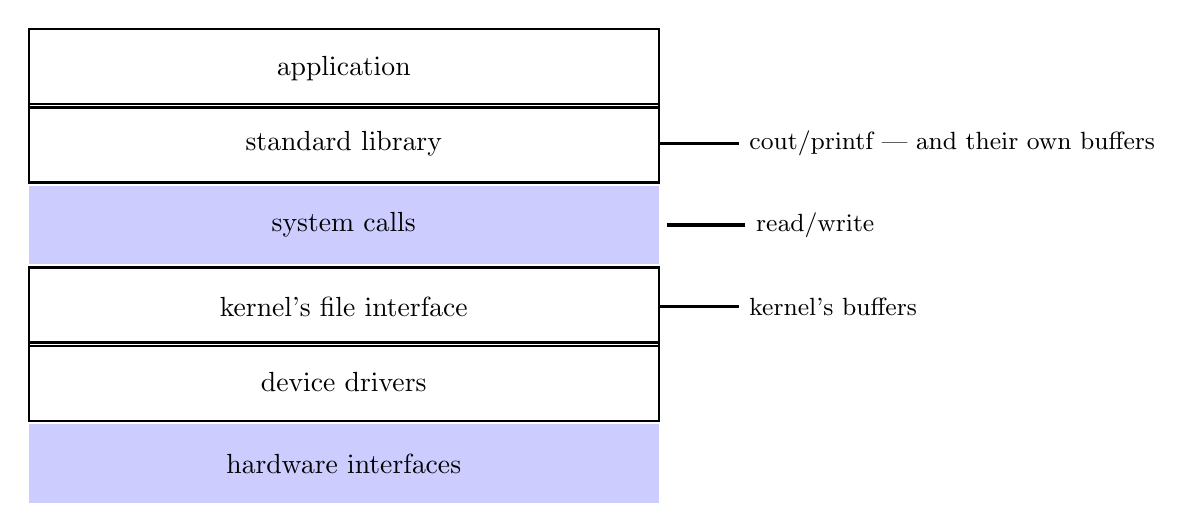
\begin{tikzpicture}
\tikzset{
    box/.style={draw,thick,minimum width=8cm,minimum height=1cm},
    thin box/.style={fill=blue!20,minimum width=8cm,minimum height=1cm,outer sep=1mm},
}
\begin{scope}[start chain=going below,node distance=-.75mm,every node/.style={on chain}]
\node[box] (application) {application};
\node[box] (library) {standard library};
\node[thin box] (syscalls) {system calls};
\node[box] (kernel file) {kernel's file interface};
\node[box] (device driver) {device drivers};
\node[thin box] (hardware) {hardware interfaces};
\end{scope}
\draw[very thick] (kernel file.east) -- ++(1cm,0cm) node[right,font=\small] {kernel's buffers};
\draw[very thick] (syscalls.east) -- ++(1cm,0cm) node[right,font=\small] {read/write};
\draw[very thick] (library.east) -- ++(1cm,0cm) node[right,font=\small] {cout/printf --- and their own buffers};
\end{tikzpicture}
\end{frame}
